\chapter{Množice}

\section{In še množice}

Zadnji izmed vgrajenih podatkovnih tipov, ki si ga moramo pogledati, so množice. Množice za predstavitev podatkov uporabljamo takrat, ko želimo, da posamezen podatek obravnavamo največ enkrat. Ker nam Python poleg tega nad množicami omogoča izvedbo osnovnih operacij, kot so unija, presek in razlika, množice zelo spominjajo na matematične množice. 

\section{Uporaba množic}

Množice podobno kot slovarje zapisujemo v zavite oklepaje, znotraj katerih naštejemo elemente. Množico elementov 1, 2 in 3, bi torej naredili takole:
\begin{lstlisting}[language=Python]
>>> mnozica = {1,2,3}
>>> mnozica
{1, 2, 3}
>>> type(mnozica)
<class 'set'>
\end{lstlisting}
Kljub temu, da množice uporabljajo podoben zapis kot slovarji, ju Python med seboj brez problemov loči, saj slovarji za razliko od množic vsebujejo pare ključ: vrednost. Do težave pride le takrat, ko je množica oziroma slovar prazen. Do praznega slovarja pridemo tako, da podamo zavite oklepaje brez elementov:
\begin{lstlisting}[language=Python]
>>> slovar = {}
>>> slovar
{}
>>> type(slovar)
<class 'dict'>
\end{lstlisting}
Do prazne množice pridemo z uporabo funkcije \texttt{set}, ki jo pokličemo brez argumentov:
\begin{lstlisting}[language=Python]
>>> mnozica = set()
>>> mnozica
set()
>>> type(mnozica)
<class 'set'>
\end{lstlisting}

\section{Omejitve pri uporabi množic}

Elementi množic imajo zelo podobne omejitve kot ključi slovarji, za katere prav tako velja, da lahko posamezno vrednost vsebujejo največ enkrat. Prav tako kot za ključe slovarjev tudi za množice velja, da lahko vsebujejo le nespremenljive podatkovne tipe. 

Množice predstavljajo neurejeno strukturo, kar pomeni, da vrstni red elementov množice ni pomemben in tudi ni določen. Elementi torej niso vezani na indekse, zato množic ne moremo indeksirati in nad njimi delati rezine:
\begin{lstlisting}[language=Python]
>>> mnozica = {1,2,3}
>>> mnozica[0]
TypeError: 'set' object is not subscriptable
\end{lstlisting}
Prav tako nad množicami ne moremo izvajati aritmetičnih operacij, kot smo jih npr. lahko izvajali nad nizi:
\begin{lstlisting}[language=Python]
>>> {1,2,3}*3
TypeError: unsupported operand type(s) for *: 'set' and 'int'
>>> {1,2,3} + {4,5,6}
TypeError: unsupported operand type(s) for +: 'set' and 'set'
\end{lstlisting}

\section{Osnovne operacije nad množicami}

Kaj pa pravzaprav potem z množicami sploh lahko počnemo. Ko množico enkrat imamo se lahko čez njo sprehajamo z zanko \texttt{for}:
\begin{lstlisting}[language=Python]
>>> mnozica = {1,2,3}
>>> for element in mnozica:
	print(element)
1
2
3
\end{lstlisting} 
Poleg tega lahko preverjamo ali množica določen element vsebuje (ali ne) z operatorjema vsebovanosti:
\begin{lstlisting}[language=Python]
>>> mnozica = {1,2,3}
>>> 1 in mnozica
True
>>> 2 not in mnozica
False
>>> 4 in mnozica
False
\end{lstlisting}

Številu elementov v množici pravimo tudi moč množice, do katere pridemo enostavno s klicem vgrajene funkcije \texttt{len}
\begin{lstlisting}[language=Python]
>>> len({1,2,3})
3
\end{lstlisting}

\begin{zgled}
Napiši funkcijo \texttt{razlicni}, ki kot argument sprejme niz, kot rezultat pa vrne število različnih znakov, ki v nizu nastopajo
\end{zgled}
\begin{resitev}
Najprej bomo niz pretvorili v množico s funkcijo \texttt{set}. Ker množica posamezen element vsebuje največ enkrat, se bomo s tem znebili vseh potencialnih ponovitev znakov. Potem samo še izračunamo in vrnemo moč množice.
\begin{lstlisting}[language=Python,numbers=left]
def razlicni(niz):
    mnozica = set(niz) # odstranitev duplikatov
    return len(mnozica) # moc mnozice
\end{lstlisting}
\end{resitev}

Tudi primerjalni operatorji so zdaj prilagojeni matematični interpretaciji množic. Ali je prva množica podmnožica druge, lahko npr. ugotovimo z operatorjem \texttt{<=}:
\begin{lstlisting}[language=Python]
>>> {1,2,3} <= {1,2,3,4}
True
\end{lstlisting}

\section{Presek, unija in razlika}

Primeri najbolj tipičnih operacij, ki jih prikazujejo diagrami na sliki \ref{img:mnozice}, so seveda presek (\texttt{A \& B}), unija (\texttt{A | B}) in razlika (\texttt{A - B}).
\begin{figure}
    \centering
    \begin{tabular}{cc}
    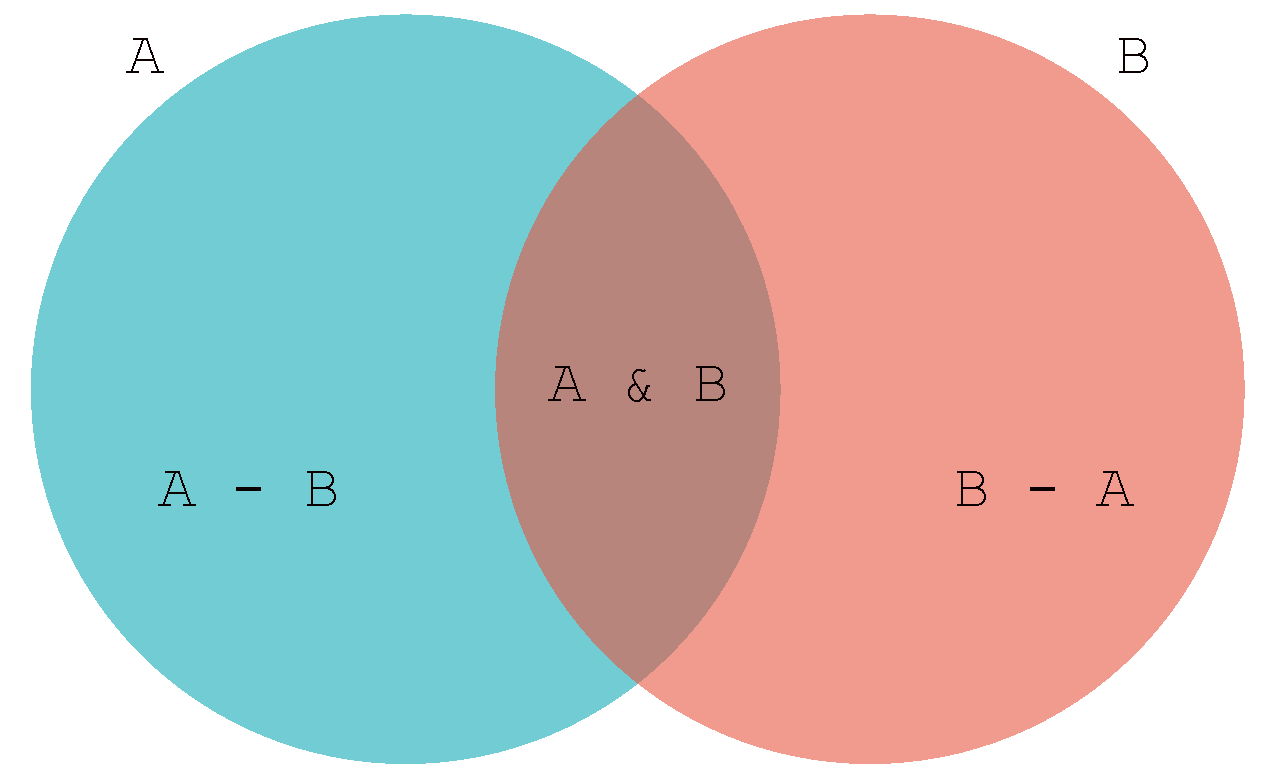
\includegraphics[width=0.45\linewidth]{img/mnozice1.pdf} & 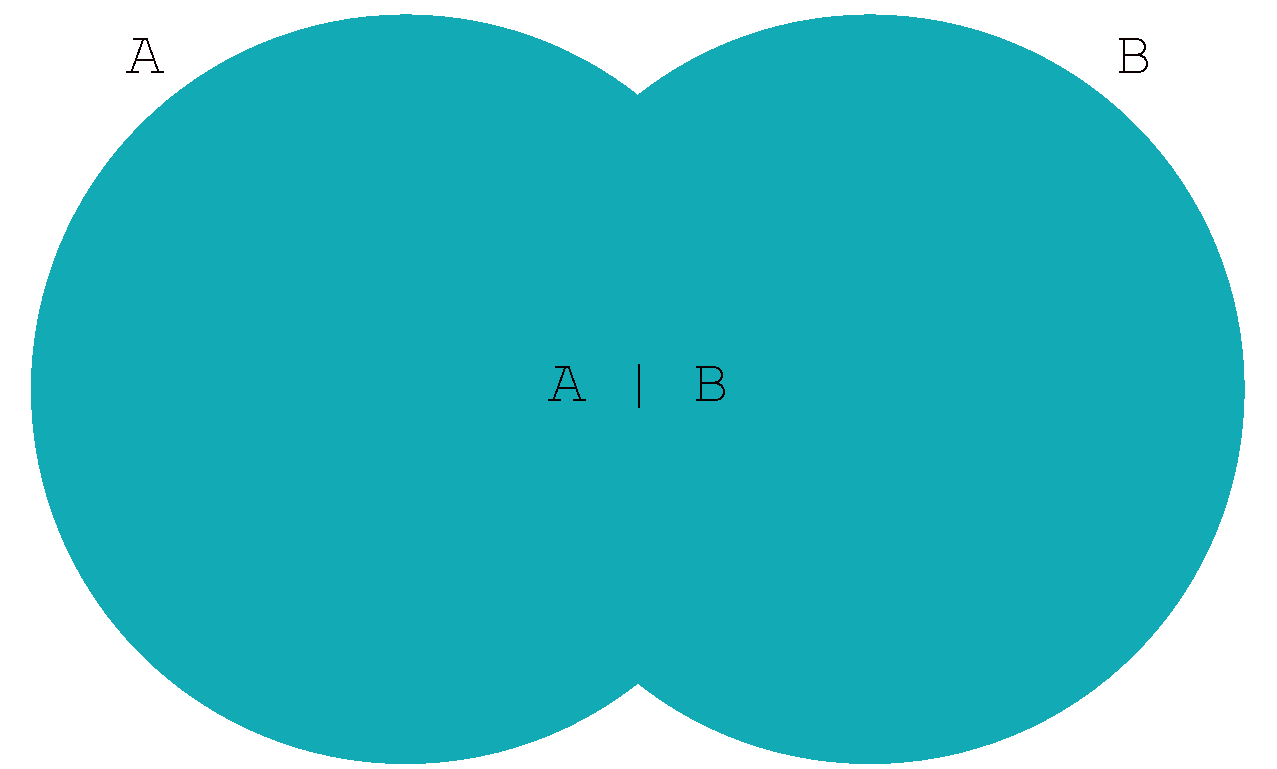
\includegraphics[width=0.45\linewidth]{img/mnozice2.pdf}\\
    \end{tabular}
    \caption{Vennova diagrama, ki ponazarjata osnovne operacije nad množicami. Slika na levi prikazuje razliko (\texttt{A-B} in \texttt{B-A}) in presek (\texttt{A \& B}) med množicama \texttt{A} in \texttt{B}. Slika na desni prikazuje unijo (\texttt{A | B}) med množicama \texttt{A} in \texttt{B}}
    \label{img:mnozice}
\end{figure}
Primer uporabe gornjih operacij je sledeč:
\begin{lstlisting}[language=Python]
>>> {1,2,3} & {3,4,5} # presek
{3}
>>> {1,2,3} | {3,4,5} # unija
{1,2,4,5}
>>> {1,2,3} - {3,4,5} # razlika
{1,2}
\end{lstlisting}

\section{Metode množic: dodajanje in brisanje elementov}
Dodajanje elementa v množico lahko izvedemo z uporabo metode \texttt{add}, ki kot argument sprejme element, ki ga želimo dodati:
\begin{lstlisting}[language=Python]
>>> mnozica = {1,2,3}
>>> mnozica.add(4)
>>> mnozica
{1, 2, 3, 4}
\end{lstlisting}
V primeru, da dodajamo element, ki v množici že obstaja, metoda ne naredi ničesar. Dodajanje bi lahko izvedli tudi z operatorjem \texttt{|=}, ki naredi unijo množice z neko drugo množico. V tem primeru lahko dodamo več elementov naenkrat:
\begin{lstlisting}[language=Python]
>>> mnozica = {1,2,3}
>>> mnozica |= {4,5}
>>> mnozica
{1, 2, 3, 4, 5}
\end{lstlisting}

Brisanje elementov iz množice vršimo z metodo \texttt{remove}. Ta v primeru neobstoja elementa vrne napako. Uporabimo lahko tudi metodo \texttt{discard}, ki v primeru neobstoja napake ne vrne, sicer pa deluje enako kot metode remove:
\begin{lstlisting}[language=Python]
>>> mnozica = {1,2,3}
>>> mnozica.remove(3)
>>> mnozica
{1, 2}
>>> mnozica.remove(3)
KeyError: 3
>>> mnozica.discard(2)
>>> mnozica
{1}
>>> mnozica.discard(2)
\end{lstlisting}
Podobno kot prej, lahko uporabimo tudi operator \texttt{-=}, ki naredi razliko med množico in neko drugo množico in to priredi izhodiščni množici:
\begin{lstlisting}[language=Python]
>>> mnozica = {1,2,3}
>>> mnozica -= {2,3}
>>> mnozica
{1}
\end{lstlisting}

\section{Zgled uporabe množic}
Ker so bili sprotni zgledi v tem poglavju relativno skopi, bomo to nadoknadili z malo daljšim zgledom, s katerim bomo povadili tudi slovarje in mogoče še kaj. 

Zamislimo si, da bi radi opazovali omrežje prijateljev oziroma povezanost ljudi preko relacije \emph{prijateljstvo}, bodisi v resničnem ali pa virtualnem življenju. Tako omrežje lahko predstavimo z \emph{neusmerjenim grafom}, v katerem vozlišča predstavljajo imena oseb, povezave med vozlišči pa prijateljstva med osebami. Te povezave so neusmerjene, saj prijateljstvo deluje v obe smeri: če je oseba 1 prijatelj osebe 2, je tudi oseba 2 prijatelj osebe 1. Primer grafa prijateljstev prikazuje slika \ref{img:prijatelji}.
\begin{figure}
    \centering
    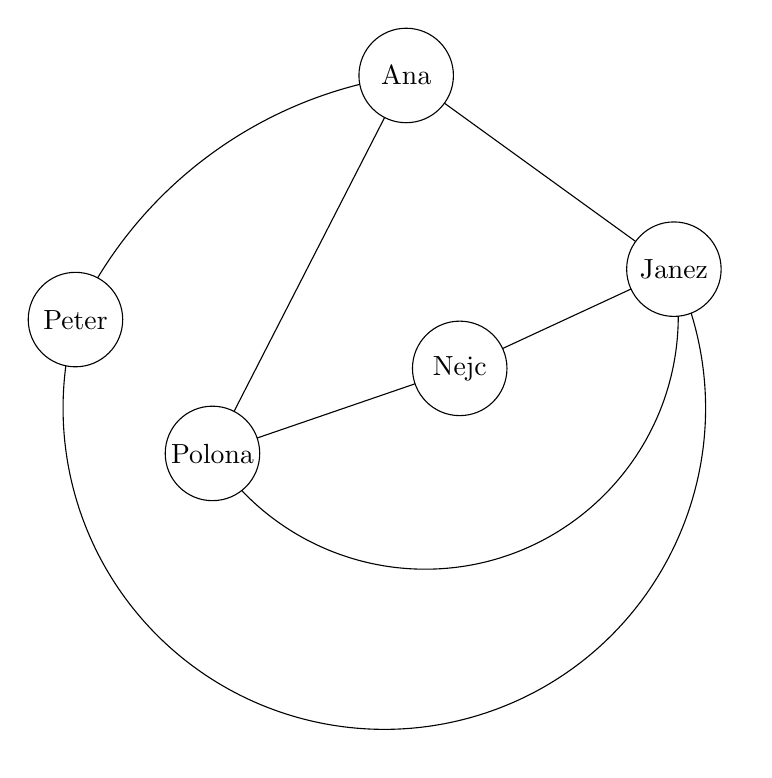
\begin{tikzpicture}[scale=0.2]
        \tikzstyle{every node}+=[inner sep=0.5pt]
        \draw [black] (32.3,-4.5) circle (3);
        \draw (32.3,-4.5) node {Ana};
        \draw [black] (11.3,-20) circle (3);
        \draw (11.3,-20) node {Peter};
        \draw [black] (20,-28.5) circle (3);
        \draw (20,-28.5) node {Polona};
        \draw [black] (35.7,-23.1) circle (3);
        \draw (35.7,-23.1) node {Nejc};
        \draw [black] (49.3,-16.8) circle (3);
        \draw (49.3,-16.8) node {Janez};
        \draw [black] (12.706,-17.352) arc (148.85774:104.00397:27.119);
        %\fill [black] (29.35,-5.06) -- (28.46,-4.77) -- (28.7,-5.74);
        \draw [black] (21.37,-25.83) -- (30.93,-7.17);
        %\fill [black] (30.93,-7.17) -- (30.12,-7.65) -- (31.01,-8.11);
        \draw [black] (32.86,-24.08) -- (22.84,-27.52);
        %\fill [black] (22.84,-27.52) -- (23.76,-27.74) -- (23.43,-26.79);
        \draw [black] (46.87,-15.04) -- (34.73,-6.26);
        %\fill [black] (34.73,-6.26) -- (35.09,-7.13) -- (35.67,-6.32);
        \draw [black] (38.42,-21.84) -- (46.58,-18.06);
        %\fill [black] (46.58,-18.06) -- (45.64,-17.94) -- (46.06,-18.85);
        \draw [black] (49.578,-19.783) arc (-0.02318:-136.44145:16.075);
        %\fill [black] (49.58,-19.78) -- (49.08,-20.58) -- (50.08,-20.58);
        \draw [black] (50.395,-19.59) arc (17.2079:-187.5808:20.399);
        %\fill [black] (50.39,-19.59) -- (50.15,-20.5) -- (51.11,-20.21);
    \end{tikzpicture}
    \caption{Primer grafa omrežja prijateljstev.}
    \label{img:prijatelji}
\end{figure}

Da se bomo lahko lotili nadaljnjih analiz omrežja prijateljstev, moramo tega najprej prestaviti v obliko, ki jo bomo lahko zapisali v Pythonu. V nadaljevanju bomo napisali par funkcij, ki jih bomo lahko uporabili pri posodabljanju omrežja in njegovi analizi.

\begin{zgled}
Izberi si podatkovno strukturo, ki jo boš lahko uporabil pri predstavitvi in analizi omrežja prijateljstev ter z njo predstavi omrežje na sliki \ref{img:prijatelji}. Pri izbiri strukture upoštevaj to, da želiš nad omrežjem vršiti funkcije, kot so dodajanje prijateljev, brisanje prijateljev, iskanje skupnih prijateljev, iskanje osebe z največ prijatelji ipd.
\end{zgled}
\begin{resitev}
Omrežje bi lahko predstavili na različne načine, a vendar težimo k tisti predstavitvi, ki nam bo pri nadaljnjih operacijah nad omrežjem prihranila največ dela, hkrati pa bodo operacije nad omrežjem potekale kar se da hitro. Začnimo z mogoče najbolj intuitivno, a ne preveč dobro predstavitvijo, in sicer s seznamom terk. V tem primeru vsaka terka v seznamu vsebuje ime osebe in seznam njenih prijateljev. Omrežje s slike \ref{img:prijatelji} bi na tak način zapisali kot:
\begin{lstlisting}[language=Python]
prijatelji = [('Ana', ['Janez', 'Peter', 'Polona']),
              ('Janez', ['Ana', 'Nejc', 'Peter', 'Polona']),
              ('Nejc', ['Janez', 'Polona']),
              ('Peter', ['Ana', 'Janez']),
              ('Polona', ['Ana', 'Janez', 'Nejc'])]
\end{lstlisting}
Zakaj predstavitev ni najboljša? Zatakne se nam že pri izpisovanje vseh prijateljev podane osebe, saj že ta zahteva iskanje podane osebe s sprehodom čez (v najslabšem primeru) celoten seznam prijateljev. Če je ta seznam dolg, je lahko ta operacija časovno zelo potratna. Stvar bi lahko izboljšali, če bi namesto seznama terk uporabili kar slovar, v katerem so ključi imena oseb, vrednosti pa seznami prijateljev. Takole: 
\begin{lstlisting}[language=Python]
prijatelji = {'Ana': ['Janez', 'Peter', 'Polona'],
              'Janez': ['Ana', 'Nejc', 'Peter', 'Polona'],
              'Nejc': ['Janez', 'Polona'],
              'Peter': ['Ana', 'Janez'],
              'Polona': ['Ana', 'Janez', 'Nejc']}
\end{lstlisting}
S tem smo rešili problem iskanja prijateljev podane osebe, saj do teh pridemo z enostavnim indeksiranjem po imenu osebe, ki nas zanima. Še vedno pa je problematično npr. iskanje skupnih prijateljev dveh oseb, saj zahteva ugnezdeno zanko po seznamih prijateljev teh dveh oseb. Spet je ta operacija lahko časovno potratna, če so ti seznami dolgi, kar v socialnih omrežjih zagotovo ni izključeno. Temu problemu bi se lahko izognili tako, da prijatelje podane osebe predstavimo z množicami, nad katerimi so operacije kot je presek bolj učinkovite. Poleg tega glede na podan opis problema vrstni red prijateljev ni pomemben, posamezna oseba pa kot prijatelj druge osebe nastopa največ enkrat. Predstavitev bi bila torej sledeča:
\begin{lstlisting}[language=Python]
prijatelji = {'Ana': {'Janez', 'Peter', 'Polona'},
              'Janez': {'Ana', 'Nejc', 'Peter', 'Polona'},
              'Nejc': {'Janez', 'Polona'},
              'Peter': {'Ana', 'Janez'},
              'Polona': {'Ana', 'Janez', 'Nejc'}}
\end{lstlisting}
\end{resitev}

\begin{zgled}
Napiši funkcijo \texttt{prijatelji\_od}, ki kot argument sprejme omrežje prijateljstev in ime osebe in vrne vse prijatelje podane osebe. V primeru, da podane osebe ni v omrežju, naj funkcija to izpiše.
\end{zgled}
\begin{resitev}
Kot smo videli že prej, je zaradi izbrane predstavitve omrežja, iskanje prijateljev podane osebe enostavno. Preveriti moramo samo, če oseba v omrežju obstaja.
\begin{lstlisting}[language=Python,numbers=left]
def prijatelji_od(prijatelji, oseba):
    if oseba not in prijatelji: # ali je oseba v omrezju?
        print("Ta oseba ne obstaja!")
    else:
        return prijatelji[oseba]
\end{lstlisting}
\end{resitev}

\begin{zgled}
Napiši funkcijo \texttt{dodaj\_osebo}, ki kot argument sprejme omrežje prijateljstev in ime osebe ter podano osebo doda v omrežje prijateljstev s prazno množico prijateljev.
\end{zgled}
\begin{resitev}
V omrežje bomo torej dodali novo osebo (nov ključ), na katerega bomo vezali prazno množico. Smiselno je tudi, da preverimo, če oseba v omrežju že obstaja. Ali mora funkcija vračati spremenjen slovar? Odgovor je seveda ne, saj je slovar spremenljiv podatkovni tip in se bo spreminjanje tega znotraj funkcije odražalo tudi izven funkcije.
\begin{lstlisting}[language=Python,numbers=left]
def dodaj_osebo(prijatelji, oseba):
    if oseba not in prijatelji: # dodaj samo, ce je se ni
        prijatelji[oseba] = set() # prazna mnozica
\end{lstlisting}
\end{resitev}

\begin{zgled}
Napiši funkcijo \texttt{spoprijatelji}, ki kot argument sprejme omrežje prijateljstev in imena dveh oseb, ki sta se spoprijateljili. Če sta osebi že v prijateljstvu, naj funkcija to izpiše. Če katerekoli izmed oseb še ni v omrežju, naj to osebo doda preko funkcije \texttt{dodaj\_osebo}.
\end{zgled}
\begin{resitev}
Spoprijateljevanje bomo naredili tako, da bomo prvo osebo dodali v množico prijateljev druge osebe in obratno. Pri tem lahko uporabimo metodo \texttt{add}. Še prej bomo po potrebi posamezno osebo dodali v omrežje, če je tam še ni.
\begin{lstlisting}[language=Python,numbers=left]
def spoprijatelji(prijatelji, oseba1, oseba2):
    if oseba1 not in prijatelji:
        dodaj_osebo(prijatelji, oseba1) 
    if oseba2 not in prijatelji:
        dodaj_osebo(prijatelji, oseba2) 
    
    # spoprijatelji samo, ce se nista prijatelja
    if oseba2 not in prijatelji[oseba1]:
        # dodaj oseba2 med prijatelje oseba1
        prijatelji[oseba1].add(oseba2)
        # dodaj oseba1 med prijatelje oseba2
        prijatelji[oseba2].add(oseba1)
    else:
        print("Osebi sta ze v prijateljstvu")
\end{lstlisting}
Primer klica:
\begin{lstlisting}[language=Python]
>>> spoprijatelji(prijatelji, 'Ana', 'Nejc')
>>> prijatelji
{'Ana': {'Janez', 'Peter', 'Nejc', 'Polona'}, 
 'Janez': {'Peter', 'Ana', 'Nejc', 'Polona'}, 
 'Nejc': {'Janez', 'Ana', 'Polona'}, 
 'Peter': {'Janez', 'Ana', 'Polona'}, 
 'Polona': {'Janez', 'Peter', 'Ana', 'Nejc'}}
>>> spoprijatelji(prijatelji, 'Ana', 'Nejc')
Osebi sta ze v prijateljstvu
\end{lstlisting}

\end{resitev}

\begin{zgled}
Napiši funkcijo \texttt{skregaj}, ki kot argument sprejme omrežje prijateljstev in imena dveh oseb, ki sta se skregali. Če osebi nista v prijateljstvu, naj funkcija to izpiše. Če katerekoli izmed oseb še ni v omrežju, naj funkcija to izpiše. 
\end{zgled}
\begin{resitev}
Pri skreganju bomo prvo osebo odstranili iz množice prijateljev druge osebe in obratno. Pri tem lahko uporabimo metodo \texttt{remove}. Še prej bomo preverili, če osebi sploh sta v omrežju in če sta v relaciji prijateljstva.
\begin{lstlisting}[language=Python,numbers=left]
def skregaj(prijatelji, oseba1, oseba2):
    if oseba1 not in prijatelji or oseba2 not in prijatelji:
        print("Ene izmed oseb ni v omrezju!")
        return # koncaj in ne vrni nic
    # ce oseba1 ni prijatelj oseba2, velja tudi obratno
    if oseba1 not in prijatelji[oseba2]:    
        print("Osebi nista prijatelja!")
        return # koncaj in ne vrni nic
    
    # odstrani prijateljstvo
    prijatelji[oseba1].remove(oseba2)
    prijatelji[oseba2].remove(oseba1)
\end{lstlisting}
Primer klica:
\begin{lstlisting}[language=Python]
>>> skregaj(prijatelji, 'Ana', 'Nejc')
{'Ana': {'Janez', 'Peter', 'Polona'}, 
'Janez': {'Peter', 'Ana', 'Nejc', 'Polona'}, 
'Nejc': {'Janez', 'Polona'}, 
'Peter': {'Janez', 'Ana', 'Polona'}, 
'Polona': {'Janez', 'Peter', 'Ana', 'Nejc'}}
>>> skregaj(prijatelji, 'Ana', 'Nejc')
Osebi nista prijatelja!
\end{lstlisting}
\end{resitev}

Zdaj pa se lotimo še analize omrežja.

\begin{zgled}
Napiši funkcijo \texttt{najbolj\_popularni}, ki kot argument sprejme omrežje prijateljstev in vrne ime osebe, ki ima največ prijateljev.
\end{zgled}
\begin{resitev}
Spet rešujemo nalogo z iskanjem največjega elementa v slovarju, tokrat glede na dolžino množice, ki se skriva za posameznim ključem. Rešitev se ne bo dosti razlikovala od programa, ki je iskal oznako nukleotida, ki se v nukleotidnem zaporedju pojavi največkrat.
\begin{lstlisting}[language=Python,numbers=left]
def najbolj_popularni(prijatelji):
    naj_oseba = ""
    naj_prijateljev = 0
    
    for oseba in prijatelji: # sprehod cez kljuce
        prijateljev = len(prijatelji[oseba]) # stevilo prijateljev
        if prijateljev > naj_prijateljev:
            naj_oseba = oseba
            naj_prijateljev = prijateljev
    return naj_oseba
\end{lstlisting}
Primer klica:
\begin{lstlisting}[language=Python]
>>> najbolj_popularni(prijatelji)
'Janez'
\end{lstlisting}

Rešitev predpostavlja, da je \emph{enako najbolj popularna} samo ena oseba, kar lahko rešimo z manjšo dopolnitvijo, tako da si najbolj popularne osebe shranimo v seznam. 
\begin{lstlisting}[language=Python,numbers=left]
def najbolj_popularni(prijatelji):
    naj_osebe = []
    naj_prijateljev = 0
    
    for oseba in prijatelji: # sprehod cez kljuce
        prijateljev = len(prijatelji[oseba]) # stevilo prijateljev
        if prijateljev > naj_prijateljev:
            naj_osebe = [oseba]
            naj_prijateljev = prijateljev
        elif prijateljev == naj_prijateljev:
            naj_osebe.append(oseba)
    return naj_osebe
\end{lstlisting}
Primer klica:
\begin{lstlisting}[language=Python]
>>> spoprijatelji(prijatelji, 'Polona','Peter')
>>> najbolj_popularni(prijatelji)
['Janez', 'Polona']
\end{lstlisting}


\end{resitev}

\begin{zgled}
Napiši funkcije \texttt{skupni\_prijatelji}, \texttt{vsaj\_od\_enega} in \texttt{brez\_njegovih}. Vse tri funkcije naj prejmejo omrežje prijateljstev in dve osebi ter vrnejo njune skupne prijatelje, prijatelje vsaj od ene izmed podanih oseb ter tiste, ki so prijatelji prve osebe ne pa prijatelji druge. V primeru, da v omrežju ni obeh podanih oseb, funkcije izpišejo, da vsaj ene podane osebe v omrežju ni.
\end{zgled}
\begin{resitev}
V tej rešitvi bomo povadili uporabo preseka (skupni prijatelji), unije (vsaj od enega) ter razlike (brez njegovih). 
\begin{lstlisting}[language=Python,numbers=left]
def skupni(prijatelji, oseba1, oseba2):
    if oseba1 not in prijatelji or oseba2 not in prijatelji:
        print("Vsaj ene osebe ni v omrezju!")
    else:
        # presek
        return prijatelji[oseba1] & prijatelji[oseba2]

def vsaj_od_enega(prijatelji, oseba1, oseba2):
    if oseba1 not in prijatelji or oseba2 not in prijatelji:
        print("Vsaj ene osebe ni v omrezju!")
    else:
        # unija
        return prijatelji[oseba1] | prijatelji[oseba2]

def brez_njegovih(prijatelji, oseba1, oseba2):
    if oseba1 not in prijatelji or oseba2 not in prijatelji:
        print("Vsaj ene osebe ni v omrezju!")
    else:
        # razlika
        return prijatelji[oseba1] - prijatelji[oseba2]
\end{lstlisting}
Primer klica:
\begin{lstlisting}[language=Python]
>>> skupni(prijatelji, 'Ana', 'Janez')
{'Peter', 'Polona'}
>>> skupni(prijatelji, 'Ana', 'Jan')
Vsaj ene osebe ni v omrezju!
>>> vsaj_od_enega(prijatelji, 'Ana', 'Janez')
{'Janez', 'Peter', 'Ana', 'Nejc', 'Polona'}
>>> brez_njegovih(prijatelji, 'Ana', 'Janez')
{'Janez'}
\end{lstlisting}
\end{resitev}


\begin{zgled}
Napiši funkcijo \texttt{prijatelji\_prijateljev}, ki kot argumenta sprejme omrezje prijateljev in ime osebe ter vrne prijatelje prijateljev podane osebe, pri čemer naj izpusti prijatelje podane osebe ter podano osebo samo.
\end{zgled}
\begin{resitev}
Tokrat se bomo sprehodili čez prijatelje podane osebe z uporabo zanke \texttt{for} ter s prijatelji prijateljev dopolnili na začetku prazno množico. Potem bomo iz te množice izločili prijatelje podane osebe in osebo samo.
\begin{lstlisting}[language=Python,numbers=left]
def prijatelji_prijateljev(prijatelji, oseba):
    vsi_pp = set() #prijatelji prijateljev je na zacetku prazna
    
    # sprehod cez prijatelje osebe
    for prijatelj in prijatelji[oseba]:
        pp = prijatelji[prijatelj]
        vsi_pp |= pp # z unijo dodam prijatelje prijatelja
    # odstranim osebo
    vsi_pp.remove(oseba)
    # odstranim neposredne prijatelje osebe
    vsi_pp -= prijatelji[oseba]
    
    return vsi_pp

\end{lstlisting}
Primer klica:
\begin{lstlisting}[language=Python]
>>> prijatelji_prijateljev(prijatelji, 'Nejc')
{'Ana', 'Peter'}
\end{lstlisting}
\end{resitev}


